L'interface utilisateur est découpée en 3 parties, qui reprennent les trois fonctionnalités clé du logiciel.

\begin{figure}[!h]
  \begin{center}
  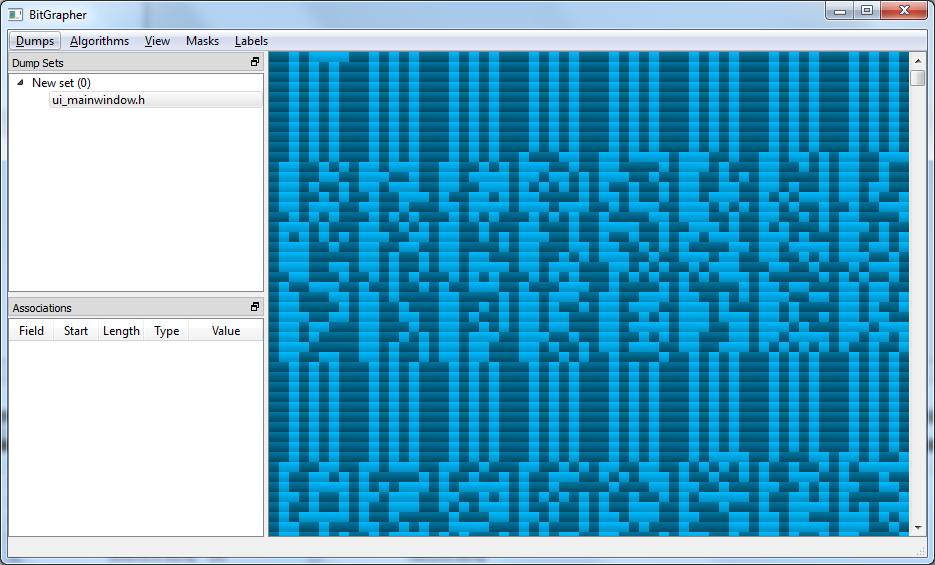
\includegraphics[width=\textwidth]{res/03-2-interface.png}
  \caption{Interface du logiciel}
  \label{03-2-interface}
  \end{center}
\end{figure}

Le premier volet (1) contient la liste des ensembles de dumps actuellement étudiés. Un dump set peut contenir plusieurs dumps, qui seront comparés entre eux.

Le second volet (2) affiche la liste des champs identifiés par l'utilisateur. Au fur et à mesure de l'analyse du dump, les données collectées permettent de comprendre la structure du fichier.

La zone d'affichage principale (3) correspond à une visualisation des données du dump, qui peut être sous la forme de texte avec un encodage choisi au préalable comme sur la figure \ref{03-2-interface}, ou bien sous forme de bitmap.

Les menus donnent accès aux différents outils d'analyse, ainsi qu'à la sauvegarde et au chargement de dumps, de dump sets ou de masques.

L'interface utilisateur est entièrement fluide et les volets peuvent être détachés ou déplacés pour que l'utilisateur puisse organiser son espace de travail comme il le souhaite.

Une description complète du logiciel est disponible dans la documentation utilisateur, où se trouvent également les adresses de télechargement de versions compilées et prêtes à l'emploi pour Windows et Linux.
